\documentclass[a4paper, 12pt]{report}
\usepackage{csquotes}
\usepackage{titlesec}
\usepackage[ngerman]{babel}
\usepackage[a4paper, left=3cm, right=3cm, top=2cm, bottom=2cm]{geometry}
\usepackage{fouriernc}
\usepackage{titlesec}
\usepackage{keystroke}

\newcommand{\makeTitleAndTable}{
    \begin{titlepage}
        \centering
        \vspace*{1.5cm}
        {\Huge Einfacher SPH Flüssigkeitssimulator mit Beschleunigter Nachbarschaftssuche\par}
        \vspace{1cm}
        {\LARGE Thierry Meiers\par}
        {\Large Bachelor Projekt\par}
        \begin{figure}[H]
            \centering
            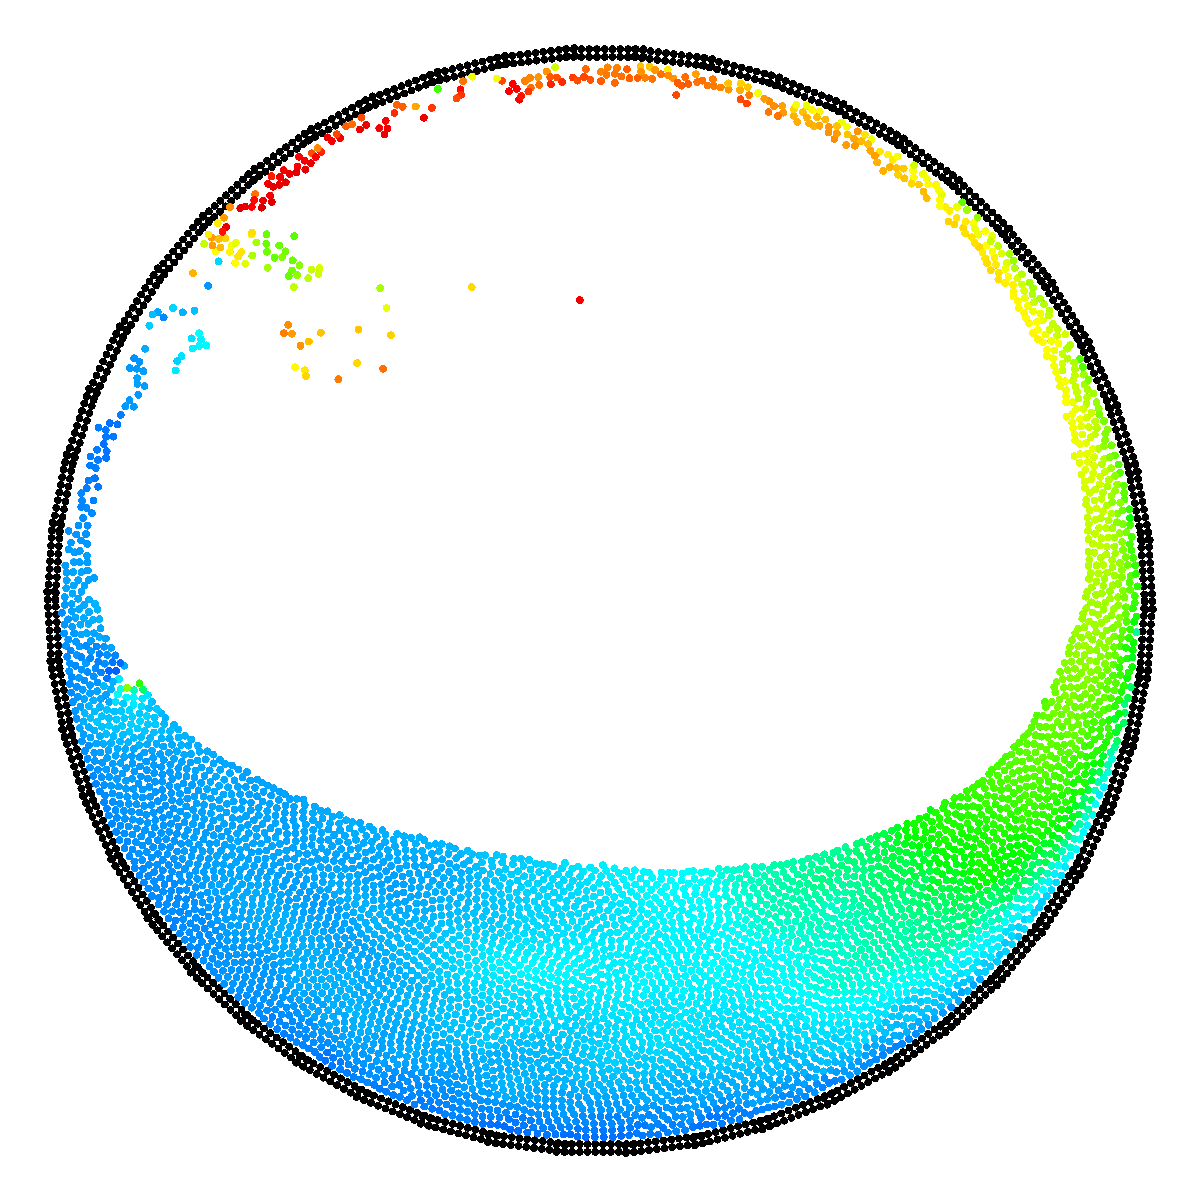
\includegraphics[width=.7\textwidth]{graphics/FirstPage.png}
        \end{figure}
        \vspace{0.5cm}
        {\large Albert-Ludwigs-Universität Freiburg\\Technische Fakultät\\Graphische Datenverarbeitung\par}
        \vfill
        {\large \today \par}
    \end{titlepage}
    \pagenumbering{gobble}
    \tableofcontents
    \clearpage
    \pagenumbering{arabic}
}

\usepackage[ngerman]{babel}
\usepackage[dvipsnames]{xcolor}
\usepackage{graphicx} 
\usepackage{microtype}
\usepackage{subcaption}
\usepackage{float}
\usepackage{parskip}
\usepackage{amsmath}
\usepackage{hyperref}
\usepackage{enumitem}

\title{Stochastic Ray Tracing}
\author{Meiers Thierry}
\date{May 2024}

\begin{document}

\makeTitleAndTable

\begin{align*}
    \frac{5}{14\pi H^2} \times
    \begin{cases}
    (2 - \frac{||position1 - position2||}{H})^3 - 4 \times (1 - \frac{||position1 - position2||}{H})^3 & \text{if } 0 \leq \frac{||position1 - position2||}{H} < 1 \\
    (2 - \frac{||position1 - position2||}{H})^3 & \text{if } 1 \leq \frac{||position1 - position2||}{H} < 2 \\
    0 & \text{otherwise}
    \end{cases}
\end{align*}

\begin{align*}
    \frac{\text{position1} - \text{position2}}{\frac{5}{14\pi H^3}} \times \text{distance} \times
    \begin{cases}
    -3 \times (2 - \frac{\text{distance}}{H})^2 + 12 \times (1 - \frac{\text{distance}}{H})^2 & \text{if } 0 \leq \frac{\text{distance}}{H} < 1 \\
    -3 \times (2 - \frac{\text{distance}}{H})^2 & \text{if } 1 \leq \frac{\text{distance}}{H} < 2 \\
    0 & \text{otherwise}
    \end{cases}
\end{align*}

\chapter{Einführung}
\chapter{Implementierung}
\chapter{Ergebnisse}
\end{document}